%!TEX program = xelatex
% 完整编译: xelatex -> biber/bibtex -> xelatex -> xelatex
\documentclass[lang=cn,11pt,a4paper]{elegantpaper}

\title{有限元第二次编程作业}
\author{W Huang}
\date{\zhtoday}


% 本文档命令
\usepackage{array}
\usepackage{float}
\usepackage{multirow}
\usepackage{amsmath}
\usepackage{amssymb}
\newcommand{\ccr}[1]{\makecell{{\color{#1}\rule{1cm}{1cm}}}}

\begin{document}

\maketitle

\section{编程第一题}

\subsection{求解设置}

求解PDE
\begin{equation}
    \left\{
        \begin{array}{l}
            -u'' = f,\quad \text{in}\;\Omega=(0,1),\\
            u(0) = u(1) = 0.
        \end{array}
    \right.
\end{equation}
取一右端项 $f\in L_\text{loc}^2(\Omega)$:
\begin{equation}
    f(x)=\frac{1}{x}.
\end{equation}
显然 $f$ 在 $0$ 处不连续,且 $f\notin L^2(\Omega)$。我们导出精确解:
\begin{equation}
    u(x)=x\ln x.
\end{equation}
注意到 $u\in H^1(\Omega)\cap C(\overline{\Omega})$。
使用非均匀网格$x_i=(i/N)^2$,取$\mathcal{P}_1$元。
使用预优共轭梯度法 (Preconditioned CG) 求解,
用超松弛迭代 (SSOR) 作为预优因子,
超松弛系数取 $2-\varepsilon$,其中 $\varepsilon=10^{-12}$。
右端项的数值积分由单元中点处的取值代替。
注意:对于 $x_0=0$ 的节点基函数 $\Phi_0$,我们知道
$\langle f, \Phi_0 \rangle$ 是发散的,
但在 Dirichlet 边界条件下,我们不需要这一项。

\subsection{编译说明}

请安装 deal.ii 及其依赖库,见 https://www.dealii.org/developer/readme.html;安装完毕后,在本文档目录下打开终端,依次运行:
\begin{lstlisting}
cd src-p1
mkdir build
cd build
cmake ..
make release
make
\end{lstlisting}
等待编译完成后,用以下命令执行测试:
\begin{lstlisting}
./elliptic 10 u
\end{lstlisting}
上述测试采用 1.1 节所述的非均匀网格,规模为 $N=2^{10}$,如果需要改变网格规模,将 \verb|10| 换成别的正整数即可。另外,如果想测试均匀网格,只需将上述命令中的 \verb|u| 删去即可。

\subsection{测试结果}

\begin{figure}[H]
    \centering
    \begin{minipage}[t]{0.48\textwidth}
        \centering
        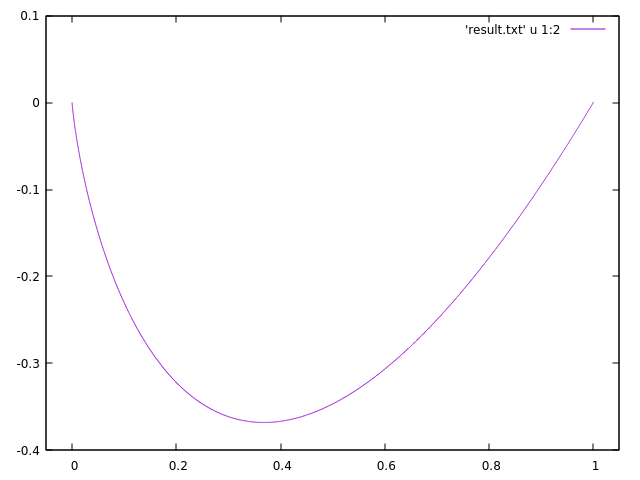
\includegraphics[width=0.9\linewidth]{png/p1-solution}
        \caption{\small $N=2^{14}$ 时非均匀网格的数值解 $u_h$}
    \end{minipage}
    \hspace{1em}
    \begin{minipage}[t]{0.48\textwidth}
        \centering
        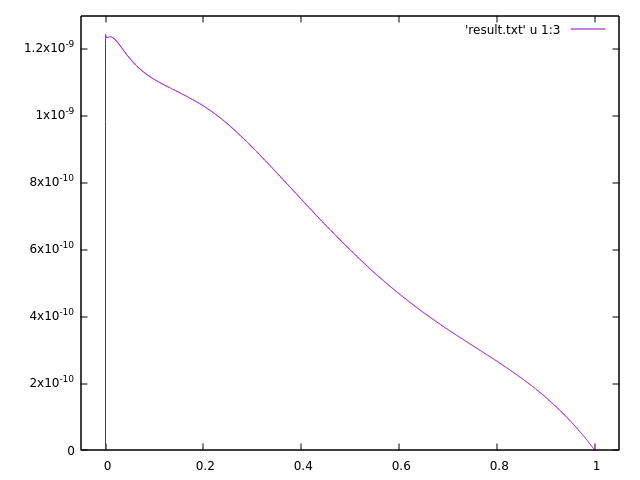
\includegraphics[width=0.9\linewidth]{png/p1-error}
        \caption{\small $N=2^{14}$ 时非均匀网格的误差 $u_h-u$}
    \end{minipage}
\end{figure}

可以看到,误差集中在奇异点附近。

\begin{table}[H]
    \centering
    \begin{tabular}{|c|c|c|c|c|c|c|c|}
    \hline
    单元数量                    & $2^{14}$ & 阶数 & $2^{15}$ & 阶数 & $2^{16}$ & 阶数 & $2^{17}$ \\ \hline
    $||u-u_h||_{L_2}$      & 1.90e-09     & 1.92 & 5.02e-10     & 1.51 & 1.76e-10     & 2.16 & 3.95e-11     \\ \hline
    $||u-u_h||_{L_\infty}$ & 2.91e-09     & 2.00 & 7.30e-10     & 1.59 & 2.42e-10     & 1.18 & 1.07e-10     \\ \hline
    $||u-u_h||_{H_1}$      & 1.60e-04     & 0.96 & 8.24e-05     & 0.96 & 4.25e-05     & 0.96 & 2.19e-05     \\ \hline
    CG 迭代次数            & 14 & & 16 & & 17 & & 19\\    
\hline
    装配耗时 (s)           & 0.019         &      & 0.035          &      & 0.072           &      & 0.15     \\ \hline
    求解耗时 (s)           & 0.0051         &      & 0.010          &      & 0.024           &      & 0.048     \\ \hline
    \end{tabular}
    \caption{\small 预优共轭梯度法,预优因子:SSOR,超松弛系数:$2-\varepsilon\;(\varepsilon=10^{-12})$}
\end{table}

由于网格尺寸太细,在机器精度的限制下,$L_2$ 和 $L_\infty$ 范数已经无法继续下降。另外可以看到,SSOR 作为预优因子效果非常好,随着网格加密,CG 迭代次数基本不会增加。换言之,当超松弛系数趋近于 $2$ 时,在 SSOR 的作用下,迭代矩阵的条件数与网格尺寸几乎无关。

刚度矩阵条件数(二范数下)的数值结果如下,数值结果支持 $\kappa(A)\sim O(N^3)$:

\begin{table}[H]
    \centering
    \begin{tabular}{|c|c|c|c|c|c|c|c|}
    \hline
    单元数量                    & $256$ & 阶数 & $512$ & 阶数 & $1024$ \\ \hline
  $\kappa(A)$            & 1.93116e+06 & 2.99 & 1.53591e+07 & 3.00 & 1.22513e+08\\    \hline
    \end{tabular}
    \caption{\small 刚度矩阵的二范数条件数,即 $\kappa(A)=||A||_2\cdot ||A^{-1}||_2$}
\end{table}

为了测试刚度矩阵的条件数对求解性能的影响,我们不使用预优因子再进行一次测试。与预优 CG 相比,朴素 CG 的求解性能大大降低,我们只好将网格规模减小以进行测试。

\begin{table}[H]
    \centering
    \begin{tabular}{|c|c|c|c|c|c|c|c|}
    \hline
    单元数量                    & $2^{12}$ & 增长率 & $2^{13}$ & 增长率 & $2^{14}$ \\ \hline
    CG 迭代次数            & 42996 & 2.86 & 122781 & 2.85 & 350164\\    
\hline
    装配耗时 (s)           & 0.005          &      & 0.01           &      & 0.02     \\ \hline
    求解耗时 (s)           & 0.49          &      & 2.35           &      & 12.7     \\ \hline
    \end{tabular}
    \caption{\small 朴素共轭梯度法}
\end{table}

\section{编程第二题}

\subsection{求解设置}

求解PDE
\begin{equation}
    \left\{
        \begin{array}{l}
            -u'' + u = f,\quad \text{in}\;\Omega=(0,1),\\
            u'(0) = u'(1) = 0.
        \end{array}
    \right.
\end{equation}
取精确解:
\begin{equation}
    u(x)=\cos(\pi x).
\end{equation}
导出右端项:
\begin{equation}
    f(x)=(1+\pi^2)\cos(\pi x).
\end{equation}
网格为均匀网格 $\mathcal{T}_1,...,\mathcal{T}_5$,其剖分节点为
\begin{equation}
    0=x_{j,0}<x_{j,1}<\cdots<x_{j,N_j}=1,
\end{equation}
其中 $x_i=i/N_j,\;N_j=2^{2j+5}$。
求解器使用 deal.ii 提供的 \verb|PreconditionSOR|,
松弛系数取 $1.0$,从而等价于 Gauss-Seidel 迭代法。

对于一些简单的积分,我们直接计算。我们记
\begin{equation}
    s(j,k)=\left\{
        \begin{array}{ll}
            1, & k=0 \; \text{or} \; k=N_j,\\
            2, & \text{otherwise},
        \end{array}
    \right.
\end{equation}
有梯度积分公式:
\begin{align}
    (\nabla \phi_{(j,k)}, \nabla \phi_{(j,k)}) &= s(j,k)N_j, \\
    (\nabla \phi_{(j,k)}, \nabla \phi_{(j,k\pm 1)}) &= -N_j, \\
    (\nabla \phi_{(j+p,4^pk)}, \nabla \phi_{(j,k)}) = (\nabla \phi_{(j,k)}, \nabla \phi_{(j+p,4^pk)}) &= s(j,k)N_j, \\
    (\nabla \phi_{(j+p,4^p(k\pm 1))}, \nabla \phi_{(j,k)}) = (\nabla \phi_{(j,k)}, \nabla \phi_{(j+p,4^p(k\pm 1))}) &= -N_j, \\
    \text{otherwise:} \quad (\nabla \phi_{(j,k)}, \nabla \phi_{(l,m)}) &= 0.
\end{align}
以及\textbf{同层}基函数的积分公式:
\begin{align}
    (\phi_{(j,k)}, \phi_{(j,k)}) &= \frac{s(j,k)}{3N_j}, \\
    (\phi_{(j,k)}, \phi_{(j,k\pm 1)}) &= \frac{1}{6N_j}, \\
    \text{otherwise:} \quad (\phi_{(j,k)}, \phi_{(j,m)}) &= 0.
\end{align}
两个\textbf{不同层}节点基函数相乘的积分值算起来比较麻烦,
我们直接用两点高斯求积公式(具有三阶代数精度)。
对于右端项数值积分,我们把每个积分区间划分成长度为 $1/N_5$ 的小区间,
在每个小区间上用中点处的值代替积分值,然后将小区间积分值累加。


\subsection{编译说明}

请安装 deal.ii 及其依赖库,见 https://www.dealii.org/developer/readme.html;安装完毕后,在本文档目录下打开终端,依次运行:
\begin{lstlisting}
cd src-p2
cd GS
mkdir build
cd build
cmake ..
make release
make
./GS
\end{lstlisting}
即可测试在 $\mathcal{T}_5$ 上的 Gauss-Seidel 迭代。重新在本文档目录下打开终端,依次运行:
\begin{lstlisting}
cd src-p2
cd bigGS
mkdir build
cd build
cmake ..
make release
make
./bigGS
\end{lstlisting}
即可测试在 $\mathcal{T}_1,...,\mathcal{T}_5$ 上的 big Gauss-Seidel 迭代。

\subsection{测试结果}

起初,我们使用了 big Gauss-Seidel 迭代,取得了如下结果。

\begin{figure}[H]
    \centering
    \begin{minipage}[t]{0.48\textwidth}
        \centering
        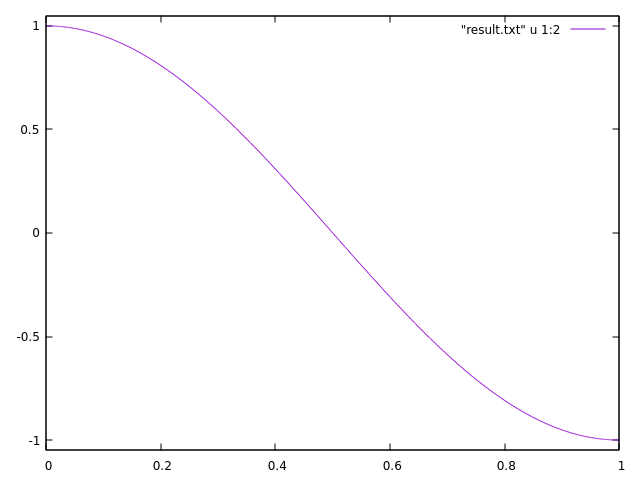
\includegraphics[width=0.9\linewidth]{png/p2-solution}
        \caption{\small big Gauss-Seldel 的数值解}
    \end{minipage}
    \hspace{1em}
    \begin{minipage}[t]{0.48\textwidth}
        \centering
        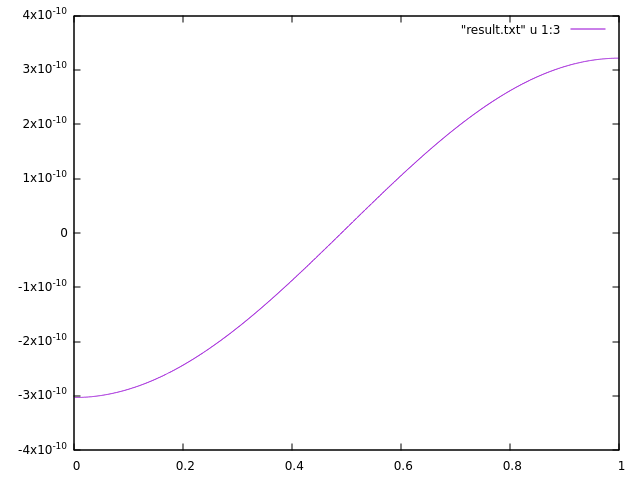
\includegraphics[width=0.9\linewidth]{png/p2-error}
        \caption{\small big Gauss-Seldel 的误差}
    \end{minipage}
\end{figure}

我们计算误差函数的离散 $L_2$ 范数,即
\begin{equation}
    ||e_h|| = \sqrt {\frac{1}{N_5+1} \sum_{k=0}^{N_5} e_h^2(x_{5,k})}.
\end{equation}
结果如下表。然而,Gauss-Seidel 的计算时间过长,
我们不愿浪费计算资源继续计算,
故在超过 4h 之后将计算进程终止。
另外,我们也尝试
将 $\mathcal{T}_1,...,\mathcal{T}_5$ 五层网格离散出的 big 方程组
用 symmetric SSOR 求解,结果一并列出。

\begin{table}[H]
    \centering
    \begin{tabular}{|c|c|c|c|c|c|c|c|}
    \hline
                        & 离散 $L_2$ 误差 & 迭代次数 & 求解耗时 \\ \hline
    Gauss-Seidel            &  &  & >4h \\
\hline
    big Gauss-Seidel           & 2.21e-10 & 316344 & 211s\\ \hline
    big symmetric SSOR     &   2.22e-10 & 41060 & 47s\\ \hline
    \end{tabular}
    \caption{\small GS 和 big GS 的效率对比}
\end{table}

\appendix
%\appendixpage
\addappheadtotoc

\end{document}
